\documentclass[10pt]{article}
\usepackage[T1]{fontenc}
\usepackage[francais]{babel}
\usepackage{array}
\usepackage{shortvrb}
\usepackage{listings}
\usepackage[fleqn]{amsmath}
\usepackage{amsfonts}
\usepackage{fullpage}
\usepackage{enumerate}
\usepackage{graphicx}             % import, scale, and rotate graphics
\usepackage{subfigure}            % group figures
\usepackage{alltt}
\usepackage{url}
\usepackage{indentfirst}
\usepackage{eurosym}
\usepackage{amsmath} 
\usepackage{float}
\usepackage{caption}

%Définition du c pour les "listings"
\usepackage{listings}
\usepackage{xcolor}
\definecolor{mGreen}{rgb}{0,0.6,0}
\definecolor{mGray}{rgb}{0.5,0.5,0.5}
\definecolor{mPurple}{rgb}{0.58,0,0.82}
\definecolor{backgroundColour}{rgb}{0.95,0.95,0.92}

\lstdefinestyle{CStyle}{
    backgroundcolor=\color{backgroundColour},   
    commentstyle=\color{mGreen},
    keywordstyle=\color{magenta},
    numberstyle=\tiny\color{mGray},
    stringstyle=\color{mPurple},
    basicstyle=\footnotesize,
    breakatwhitespace=false,         
    breaklines=true,                 
    captionpos=b,                    
    keepspaces=true,                 
    numbers=left,                    
    numbersep=5pt,                  
    showspaces=false,                
    showstringspaces=false,
    showtabs=false,                  
    tabsize=2,
    language=C
}


%\usepackage[french,onelanguage,ruled,vlined]{algorithm2e}
%\usepackage{clrscode3e}
%\usepackage{algorithm, algpseudocode}
%\usepackage{tabular}
\usepackage[utf8]{inputenc}
\usepackage{clrscode3e}
%\usepackage{algpseudocode}

% changement de la numerotation
\setcounter{secnumdepth}{5}
%\renewcommand{\thechapter}{\Alph{chapter}}
%\renewcommand{\thesection}{\Roman{section})}
%\renewcommand{\thesubsection}{\arabic{subsection})}


%\title{\textbf{INFO2050 : Rapport numéro un programmation avancée}}
%\author{Antoine Sadzot}
%\date{30-10-17}
\begin{document}
\begin{titlepage}

   \begin{figure}[htbp]
      \centering
      
\includegraphics{uliege-logo-couleurs-300.jpg}
   \end{figure}
  	
  	\hfill

	\begin{center}
		\vfill
		\textbf{
		\Huge{INFO2050-1 - Programmation Avancée}}\\
		\bigskip
		\huge{Projet 3: Mise en page automatique d'une bande dessinée}\\
		\bigskip %saut de ligne
		\smallskip
		\Large{Aliaksei Mazurchyk\\Antoine Sadzot}\\
		\bigskip
		\smallskip
		\large{\today}\\%date
		\vfill
		\large{Université de Liège}
	\end{center}
\end{titlepage}
\clearpage
\clearpage

\section{Algorithme par programmation dynamique}
\subsection{Approche par recherche exhaustive}
\subsubsection{Comic}
Pour $n$ cases, il y a $n-1$ endroits de coupe possible (entre les cases). Entre chaque case il faut choisir s'il faut passer à la ligne ou continuer. Un choix binaire donc. Il y a donc $2^{n-1}$ possibilités pour agencer $n$ cases.
\subsubsection{Seam carving}
Pour créer une couture, on part d'un pixel de la première rangée. De là, on a le choix entre trois directions pour continuer la couture à la rangée suivante. Pour avancer d'encore une rangée, on a encore le choix entre trois directions... On a donc (en prenant en compte les bords gauche et droit) une complexité $O(m*3^n)$ où m est le nombre de pixels de départ à la première rangée et n le nombre de pixels en hauteur.

\subsection{Formulation récursive de la fonction de coût}
\subsubsection{Comic}
$$
c(n) = \left\{
	\begin{array}{ll}
		cost(n) & si\ j==j \\
		E(i,j)+min(C(i-1,j-1),C(i-1,j),C(i-1,j+1)) & sinon
	\end{array}
\right.
$$
\subsubsection{Seam carving}
$$
C(i,j) = \left\{
	\begin{array}{ll}
		E(0,j) & si\ i==0 \\
		E(i,j)+min(C(i-1,j-1),C(i-1,j),C(i-1,j+1)) & sinon
	\end{array}
\right.
$$

\subsection{Graphe des appels récursifs pour un problème de petite taille}
\subsubsection{Comic}
\subsubsection{Seam carving}
Graphe des appels récursif
 \begin{figure} [h]
      \centering
      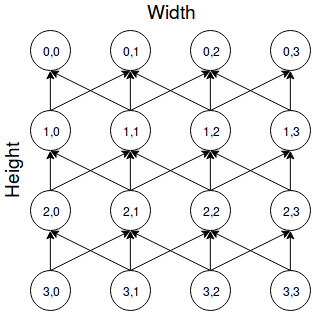
\includegraphics[scale=0.5]{GrapheSeamCarving.png}
   \end{figure}
\subsection{Algorithme des fonctions de coût}
\subsubsection{Comic}La fonction \textbf{ c(image,i,j)} permet de calculer la disposition minimale ainsi que son cout. Pour réduire les temps de calcul, cette fonction utilise la mémoïsation afin de sauvegarder la différence de largeur entre un ensemble d'images et la largeur souhaitée. Ceci ce fait en utilisant un tableau à deux dimensions (\textbf{memo} de taille $n \times n$). La sauvegarde se fait à l'intérieur de la fonction \textbf{cost(i,j,width)}.

Les résultats de découpe se fond dans la tableau \textbf{cuts}.
\begin{lstlisting}[frame=single]
c (image, i, j, memo, cuts)
	if(i>=j)
	{
		ADD i to cuts
		return cost(j,j), memo, cuts 
	}
	else
	{
		k=i
		while(true)
		{
			tmp=cost(k,j)
			if(tmp>cost(k+1,j,memo)
				k++
			else
				ADD k to cuts
				tmp += c(image, k, j, memo, cuts)
				break
		}
		return tmp, memo, cuts
	}
\end{lstlisting}
\subsubsection{Seam carving} \label{sssec:num1}
La fonction\textbf{ E(image,i,j)} est la fonction qui calcule l'énergie d'un pixel. Le tableau \textbf{energies} contient les coutures d'énergie minimales pour atteindre chaque pixel depuis la première rangée. Le tableau \textbf{moves} contient le déplacement à faire (gauche, centre, droite) pour suivre une couture de bas en haut. 
\begin{lstlisting}[frame=single]
C (image, energies, moves)
for i=0 to n
	for j=0 to m
	{
	if i==0
		energies[i,j]=E(image,i,j)
	else
		if E(image,i-1,j-1) < E(image,i-1,j)
			tmp=E(image,i-1,j-1)
		else
			tmp=E(image,i-1,j)
		if tmp < E(image,i-1,j+1)
			min=tmp
		else
			min=E(image,i-1,j+1)
		energies[i,j]=E(image,i,j)+min
		if min == E(image,i-1,j-1)			
			moves[i,j]= -1
		else if min = E(image,i-1,j)
			moves[i,j]=0
		else
			moves[i,j]=1
	}
return energies, moves
\end{lstlisting}

\subsection{Complexité en temps et en espace}
\subsubsection{Comic}
La complexité en temps de l'algorithme est $\Theta(n)$.
La complexité en espace est $\Theta(n \times (n+2))$. Les images, le tableau $n^2$ pour la mémoïsation et un tableau de découpe de taille $n$.
\subsubsection{Seam carving}
La complexité en temps de l'algorithme est $\Theta(n*m)$
La complexité en espace est $\Theta(3*n*m)$. Car il y a trois tableaux de dimension n*m. L'image en elle même, plus un tableau pour enregistrer les coutures d'énergie et un tableau pour enregistrer les déplacements à faire pour suivre une couture de bas en haut.

\section{Fonctions de réduction et d'augmentation d'images}
\subsection{Choix d'implémentation}
\subsubsection{ImagewidthReduction}
Plusieurs fonctions auxiliaires sont utilisées pour réduire la taille d'une image.
La fonction \textbf{pixelEnergy} renvoie l'énergie calculée d'un pixel appartenant à une image donnés en argument.

Cette fonction est utilisée par la fonction \textbf{seams}, qui est une implémentation de l'algorithme de la section \ref{sssec:num1}. 

Ensuite, la fonction \textbf{selectSeam} parcourt le tableau d'énergies généré à la fonction précédente pour déterminer la couture d'énergie la plus faible.

Dans la fonction principale, une boucle correspond au nombre de pixels à diminuer sur la largeur de l'image. Deux images temporaires sont utilisées. Initialement, la première image a une largeur identique à l'image originelle. La seconde image est moins large d'un pixel. A chaque itération, une couture minimale est déterminée sur la première image temporaire. La seconde image temporaire est générée en retirant les pixels de la couture. A la fin de l'iteration, la première image est supprimée et remplacée par la seconde.

\subsubsection{ImagewidthExpansion}
La fonction a un fonctionnement similaire à l'image précédente. Cependant, conformément aux consignes, l'image est élargie par "lots" de k itérations correspondant à maximum 20\% de la largeur de l'image. Lors de ces itérations, un tableau contenant les k coutures d'énergie minimales sur l'image originale est généré. Pour ce faire on reprend la fonction \textbf{seams} décrite précédemment. Mais elle est modifiée pour pouvoir rejeter systématiquement les coutures précédemment générées. Dans l'implémentation actuelle, une nouvelle image temporaire de largeur +1 est générée à chaque itération (et donc à chaque nouvelle couture déterminée). Idéalement, cette nouvelle image pourrait n'être créée qu'une fois toutes les coutures déterminées.
Si le nombre de pixels à ajouter est plus important que 20\%, on recommence les étapes décrites au dessus. Jusqu'à ce que le résultat ait la largeur choisie.

\subsection{Complexité en temps et en espace}

\subsubsection{ImageWidthReduction}
\textbf{Complexité en espace}. En plus de l'image originelle, deux autres images avec un écart de largeur égal à 1 sont générées pour les calculs. En fonction des itérations, leur largeur évolue entre la largeur originelle et la largeur cible. A ces deux images s'ajoutent le tableau contenant les coutures et le tableau contenant les déplacements. Les largeurs des deux tableaux évoluent comme les images. Et à cela s'ajoute un vecteur de taille "n", contenant les numéros de colonne des pixels impliqués dans la couture sélectionnée.
	La complexité en espace est donc maximale au début de la fonction : $\theta(4(nm) + n(m-1) + n)$ = $\theta(5nm)$
\textbf{Complexité en temps}. Pour diminuer ou augmenter une image de 1px en largeur la complexité en temps est la suivante :
L'image est parcourue une fois pour déterminer les coutures($\theta(n*m)$). Elle est ensuite parcourue en largeur et en hauteur pour déterminer la couture d'énergie minimale ($\theta(n+m)$). L'image est ensuite parcourue une nouvelle fois pour générer une nouvelle image. Comme la nouvelle image contient une colonne de moins, le parcours est impacté. Donc la complexité de ce parcours est $\theta(n*m - n)$.

On a donc au total une complexité $\theta(2n*m + m)$.

 Il faut maintenant prendre en compte le nombre k d'itérations à effectuer pour modifier l'image de k pixels en largeur. En faisant attention que la taille des tableaux diminue à chaque itération.
$$
 	T_{n,m,k} = \sum\limits_{i=0}^{k} 2n(m-i) + m-i 
$$
$$
 	= (2n + 1)\sum\limits_{i=0}^{k} (m -i)
$$
$$
 	= (2n + 1)(\sum\limits_{i=0}^{k} m - \sum\limits_{i=0}^{k} i)
$$
$$
 	= (2n + 1)(k*m - \frac{k(k+1)}{2})
$$
$$
 	= k(2n + 1)(m - \frac{(k+1)}{2})
$$
Lorsque k est négligeable par rapport à m, la complexité est proche de $\theta(2knm)$\\
\subsubsection{ImageWidthExpansion}
\textbf{Complexité en espace}. La complexité en espace est similaire à la fonction de réduction. A la différence que le vecteur contenant les coutures sélectionnées contient maintenant k*n éléments. Et l'image générée contient une colonne de plus. La complexité est donc :  $\theta(4(nm) + n(m+1) + nk)$ = $\theta(5nm + n(1 + k))$

\textbf{Complexité en temps}.
La fonction d'élargissement est un peu plus complexe, car il faut prendre en compte le parcours du tableau contenant les coutures sélectionnées au sein de la fonction \textbf{seams}.

En comptant que lorsqu'on génère une nouvelle image de largeur + 1, une colonne de plus est parcourue. La complexité est donc formulée comme tel :
$$
 	T_{n,m,k} = \sum\limits_{i=0}^{k} n(m+i)i + n + (m+i) + n(m+i) + n 
$$
Pour faciliter les calculs, on ignore les éléments $n$,$n$,$(m+i)$. On a donc :
$$
 	T_{n,m,k} = \sum\limits_{i=0}^{k} n(m+i) + \sum\limits_{i=0}^{k} n(m+i)i 
$$
$$
 	= kn(m + \frac{k + 1}{2}) + kn(m\frac{k + 1}{2} + \frac{(2k + 1)(k + 1)}{6})
$$
$$
 	= kn(m(1 + \frac{k + 1}{2}) + \frac{k + 1}{2} + \frac{2k^2 + 3k + 1}{6})
$$
La complexité obtenue est donc $\Omega(knm)$
\end{document}
